\documentclass[12pt,a4paper]{article}
\usepackage[utf8]{inputenc}
\usepackage[spanish,es-tabla]{babel}
\usepackage{geometry}
\usepackage{graphicx}
\usepackage{multirow}
\usepackage{tabularx}
\usepackage{mathptmx}
\usepackage{fancyhdr}
\usepackage{array}
\usepackage[table]{xcolor}
\usepackage{titlesec}
\usepackage{setspace}
\usepackage{microtype}
\usepackage{lastpage}
\usepackage{booktabs}
\usepackage{enumitem}
\usepackage{amsmath}
\usepackage{amsfonts}
\usepackage{amssymb}
\usepackage{listings}

\lstset{
  basicstyle=\ttfamily\scriptsize,
  backgroundcolor=\color{gray!8},
  frame=single,
  breaklines=true,
  tabsize=2,
  showstringspaces=false
}

\graphicspath{{images/}{../images/}{./}}

\geometry{
    top=4.7cm,
    bottom=2.5cm,
    left=2.5cm,
    right=2.5cm,
    headheight=3.9cm,
    headsep=0.4cm
}

\setstretch{1.15}
\setlength{\parindent}{0pt}
\setlength{\parskip}{0.45em}
\setlength{\tabcolsep}{4pt}

\titleformat{\section}
  {\normalfont\fontsize{12}{14.5}\bfseries}{\thesection.}{0.6em}{\uppercase}
\titlespacing*{\section}
  {0pt}{1.8ex plus 0.4ex minus 0.2ex}{0.6ex plus 0.2ex}

\titleformat{\subsection}
  {\normalfont\fontsize{11.5}{13.5}\bfseries}{\thesubsection.}{0.5em}{}
\titlespacing*{\subsection}
  {0pt}{1.4ex plus 0.3ex minus 0.1ex}{0.4ex plus 0.1ex}

\titleformat{\subsubsection}
  {\normalfont\fontsize{10.5}{12.5}\bfseries\itshape}{\thesubsubsection.}{0.4em}{}
\titlespacing*{\subsubsection}
  {0pt}{1.1ex plus 0.2ex minus 0.1ex}{0.3ex plus 0.1ex}

\newcolumntype{Y}{>{\centering\arraybackslash}X}
\newcolumntype{L}{>{\raggedright\arraybackslash}X}
\newcolumntype{C}{>{\centering\arraybackslash}X}

\definecolor{headerred}{RGB}{180, 0, 0}
\definecolor{darkred}{RGB}{140, 0, 0}
\definecolor{lightgraybg}{RGB}{248, 248, 248}
\definecolor{tableheader}{RGB}{232, 238, 246}

\newcommand{\docCodigo}{TI-SIGE-ENT-S2-005}
\newcommand{\docVersion}{1.0}
\newcommand{\docProceso}{DISEÑO DE SOFTWARE / EXPERIENCIA DE USUARIO UI-UX}
\newcommand{\docElaboracion}{03/09/2026}
\newcommand{\docRevision}{PENDIENTE DE REVISIÓN}
\newcommand{\docTitulo}{DISEÑO DE INTERFACES DE USUARIO, WIREFRAMES Y GUÍA DE ESTILO UX}
\newcommand{\docOrganizacion}{FACULTAD DE INGENIERÍA EN SISTEMAS, ELECTRÓNICA E INDUSTRIAL}
\newcommand{\docSubOrganizacion}{CARRERA DE INGENIERÍA DE SOFTWARE}

\newcommand{\encabezadofrecuente}{%
    \renewcommand{\arraystretch}{1.15}%
    \noindent\makebox[\textwidth][c]{%
    \begin{tabularx}{\textwidth}{|>{\centering\arraybackslash}m{2.8cm}|Y|>{\centering\arraybackslash}m{4.8cm}|}
        \hline
        \multirow{4}{2.8cm}{\centering\raisebox{-1.15cm}{
\includegraphics[width=2.5cm,height=2.0cm,keepaspectratio]{images/logo.png}}}
        & \textbf{\fontsize{9}{11}\selectfont \docOrganizacion} 
        & \textbf{\fontsize{8}{10}\selectfont CÓDIGO:} \fontsize{8}{10}\selectfont \docCodigo \\
        \cline{3-3}
        & \textbf{\fontsize{8.5}{10.5}\selectfont \docSubOrganizacion} 
        & \textbf{\fontsize{8}{10}\selectfont VERSIÓN:} \fontsize{8}{10}\selectfont \docVersion \\
        \cline{2-3}
        & \textbf{\fontsize{8}{10}\selectfont PROCESO:} \fontsize{8}{10}\selectfont \docProceso 
        & \textbf{\fontsize{8}{10}\selectfont ELABORACIÓN:} \fontsize{8}{10}\selectfont \docElaboracion \\
        \cline{2-3}
        & \textbf{\fontsize{8.5}{10.5}\selectfont \docTitulo} 
        & \textbf{\fontsize{8}{10}\selectfont ÚLTIMA REVISIÓN:} \fontsize{8}{10}\selectfont \textbf{\textcolor{darkred}{\docRevision}} \\
        \hline
    \end{tabularx}%
    }%
}

\pagestyle{fancy}
\fancyhf{}
\fancyhead[C]{\encabezadofrecuente}
\fancyfoot[C]{\fontsize{10}{12}\selectfont Página \thepage\ de \pageref{LastPage}}
\renewcommand{\headrulewidth}{0pt}

\begin{document}

\section{Título}
\textbf{Denominación del Entregable:} Sistema de Diseño UI/UX, Wireframes de Alta Fidelidad y Usabilidad (EDT 2.5)



\section{Introducción}
La interfaz gráfica del sistema \textbf{SIGE} ha sido concebida bajo principios de sobriedad institucional, accesibilidad web (WCAG 2.1 AA) y consistencia visual con la identidad de la Universidad Técnica de Ambato. Este entregable presenta el sistema de diseño basado en tonos azules y blancos, tokens de color, jerarquía tipográfica y wireframes de alta fidelidad para las vistas de Docente Elaborador, Comité de Revisión y Administrador SGC.

\section{Objetivo}

\subsection{Objetivo General}
Diseñar las interfaces de usuario interactivas y wireframes de alta fidelidad para el sistema SIGE, optimizando la experiencia de usuario, la navegación por pestañas y el cumplimiento de accesibilidad en la FISEI UTA.

\subsection{Objetivos Específicos}
\begin{enumerate}[leftmargin=1.5em, itemsep=2pt, topsep=2pt]
    \item Establecer el Design System institucional basado exclusivamente en la paleta Azul y Blanco.
    \item Elaborar los wireframes de navegación para las 3 vistas por rol (Docente, Comité y Administrador).
    \item Validar el ratio de contraste cromático bajo los estándares WCAG 2.1 AA.
\end{enumerate}

\section{Alcance}

\subsection{Límites del Diseño (In-Scope)}
\begin{itemize}[leftmargin=1.5em, itemsep=2pt]
    \item Interfaces de usuario para dispositivos de escritorio y portátiles (1366x768 a 1920x1080) y prototipado responsive.
    \item Prototipo funcional validado en \texttt{Prototipo\_SIGE/index.html}.
\end{itemize}

\subsection{Exclusiones (Out-of-Scope)}
\begin{itemize}[leftmargin=1.5em, itemsep=2pt]
    \item Animaciones 3D pesadas o interfaces para smartwatches.
\end{itemize}

\section{Definiciones}
\begin{itemize}[leftmargin=1.5em, itemsep=2pt]
    \item \textbf{Wireframe:} Representación esquemática visual de la disposición de elementos en pantalla.
    \item \textbf{Design System:} Conjunto de reglas, componentes y tokens de diseño reutilizables.
    \item \textbf{WCAG 2.1 AA:} Pautas de accesibilidad web del W3C para asegurar contraste visual y navegación accesible.
\end{itemize}

\section{Responsabilidades}
\begin{table}[htbp]
\centering
\small
\begin{tabularx}{\textwidth}{|>{\hsize=0.65\hsize\bfseries}X|>{\hsize=0.85\hsize}X|>{\hsize=1.5\hsize}X|}
    \hline
    \rowcolor{tableheader}
    Integrante & Rol en el Entregable & Responsabilidad Específica \\
    \hline
    Heidy Villavicencio & Analista / UI-UX & Diseño de componentes visuales en Figma, wireframes y tokens de color. \\
    \hline
    Andrea Vasquez & Frontend / QA & Implementación del prototipo HTML interactivo y pruebas de contraste WCAG. \\
    \hline
    Ing. Paulo Torres & Docente Tutor & Validación de usabilidad y adecuación a la dinámica académica docente. \\
    \hline
\end{tabularx}
\caption{Matriz de Responsabilidades del Entregable EDT 2.5.}
\end{table}

\section{Normativa Legal y Técnica}
\begin{itemize}[leftmargin=1.5em, itemsep=2pt]
    \item \textbf{W3C Web Content Accessibility Guidelines (WCAG) 2.1 (Nivel AA).}
    \item \textbf{Manual de Identidad Visual Corporativa UTA (2024).}
\end{itemize}

\section{Método, Políticas y Contenidos}
El sistema de diseño adopta la paleta institucional oficial de la UTA/FISEI basada en el estándar visual institucional y tokens configurados en Tailwind CSS con animaciones fluidas mediante CSS Keyframes:

\begin{figure}[htbp]
    \centering
    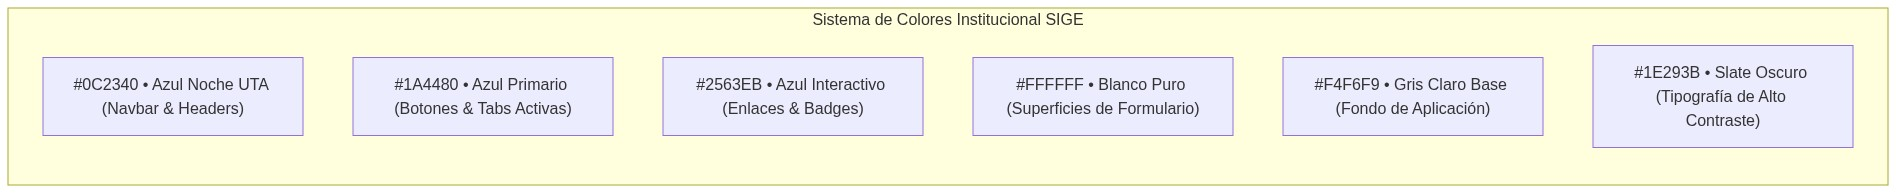
\includegraphics[width=0.85\textwidth,height=3.8cm,keepaspectratio]{images/s2_05_paleta_colores.png}
    \caption{Sistema de Colores Institucional Oficial de SIGE.}
    \label{fig:s2_05_paleta}
\end{figure}

\subsection{Tokens Cromáticos Oficiales}
\begin{itemize}[leftmargin=1.5em, itemsep=2pt]
    \item \textbf{\#00345E (Azul Institucional UTA/FISEI):} Barra de navegación superior (\textit{Navbar}), encabezados principales, botones de acción y pantalla oficial de acceso (\texttt{LoginPage.jsx}).
    \item \textbf{\#0C2340 (Azul Noche Oscuro):} Paneles laterales, menús desplegables y fondos de modales institucionales.
    \item \textbf{\#2563EB (Azul Interactivo):} Enlaces hipertextuales, badges de estado informativo y anillos de enfoque (\textit{focus ring}).
    \item \textbf{\#FFFFFF (Blanco Puro):} Superficies de formulario, fondos de modales, inputs y contenedores de tablas.
    \item \textbf{\#F4F6F9 (Gris Claro Base):} Fondo general de la aplicación web y separación de paneles laterales.
    \item \textbf{\#1E293B (Slate Oscuro):} Tipografía de cuerpo de texto de alto contraste para lectura prolongada según norma WCAG 2.1 AA.
\end{itemize}

\subsection{Tipografía y Espaciado}
\begin{itemize}[leftmargin=1.5em, itemsep=1.5pt]
    \item \textbf{Fuente Principal:} \texttt{Inter}, \texttt{-apple-system}, \texttt{BlinkMacSystemFont}, \texttt{Segoe UI}, \texttt{Roboto}, \texttt{sans-serif}.
    \item \textbf{Títulos Principales:} $16\text{ px} - 18\text{ px}$ (\texttt{font-bold}, \texttt{\#0C2340}).
    \item \textbf{Encabezados de Sección:} $13\text{ px} - 14\text{ px}$ (\texttt{font-bold}, \texttt{\#1A4480}).
    \item \textbf{Texto de Formularios y Tablas:} $12\text{ px}$ (\texttt{font-normal}, \texttt{\#1E293B}).
    \item \textbf{Metadatos y Badges:} $10\text{ px} - 11\text{ px}$ (\texttt{font-semibold}).
\end{itemize}

\section{Descripción de actividades}

\subsection{Arquitectura de Información y Wireframes por Rol}
El sistema implementa vistas dedicadas según el rol institucional:

\begin{figure}[htbp]
    \centering
    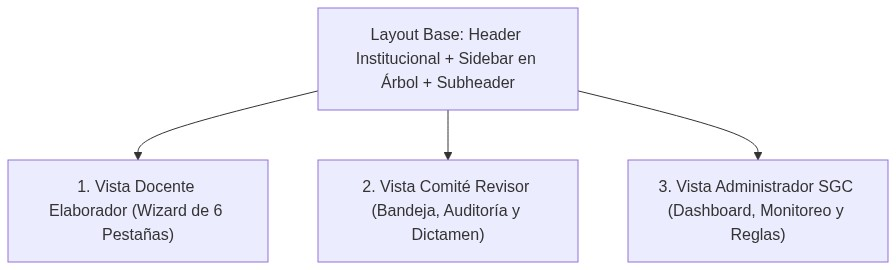
\includegraphics[width=0.82\textwidth,height=4.8cm,keepaspectratio]{images/s2_05_layout_vistas.png}
    \caption{Arquitectura de Layout y Distribución de Vistas en SIGE.}
    \label{fig:s2_05_layout}
\end{figure}

\subsection{Wireframe Vista 1: Docente Elaborador (Wizard de Pestañas y Matriz)}
\begin{lstlisting}
+----------------------------------------------------------------------------------------------------+
| [UTA] SIGE | Sistema Web de Gestion, Seguimiento y Aprobacion de Informes y Planes  [Docente: ST]   |
+----------------------------------------------------------------------------------------------------+
| Gestion Documental > DOC-2026-PLAN-014 [EN EJECUCION]    [Solicitar Modificacion Plan] [Ver PDF]   |
+----------------------------------------------------------------------------------------------------+
| MENU EN ARBOL      | [1. Datos] [2. Justificacion] [3. Matriz Cronograma] [4. Evidencias] [5. Firmas]|
| - Planes Trabajo   | +----------------------------------------------------------------------------+ |
|   * Ingresar Plan  | | 3. Matriz de Actividades y Seguimiento Continuo      [+ Anadir Actividad]  | |
|   * Mis Planes     | |----------------------------------------------------------------------------| |
| - Informes SGC     | | N  | Actividad Planificada | Desde - Hasta | Avance | Evidencia Subida |Est| |
|   * Nuevo Informe  | |  1 | Socializacion Silabo  | 01/09 - 15/09 |  100%  | [Acta_S1.pdf OK] | V | |
|   * Mis Informes   | |  2 | Direccion Proyecto    | 16/09 - 30/10 |   50%  | [Subir Evidencia]| A | |
| - Herramientas     | |  3 | Evaluaciones Primer P | 01/11 - 15/11 |    0%  | (Programada)     | G | |
|   * LanguageTool   | +----------------------------------------------------------------------------+ |
|   * MinIO Storage  | [ Regla: Subida obligatoria de evidencia al culminar cada actividad a tiempo ]|
+----------------------------------------------------------------------------------------------------+
\end{lstlisting}

\subsection{Wireframe Vista 2: Comité de Revisión (Auditoría y Cascada de Firmas)}
\begin{lstlisting}
+----------------------------------------------------------------------------------------------------+
| [UTA] SIGE | Modulo de Revision y Dictamenes (Area de Conocimiento)                [Coord. Area: PT]|
+----------------------------------------------------------------------------------------------------+
| Comision Calidad > Dictamenes SGC > DOC-2026-PLAN-014 (Docente: Steeven Toala)                     |
+----------------------------------------------------------------------------------------------------+
| BANDEJA EXPEDIENTES| AUDITORIA DE MATRIZ Y CIRCUITO DE FIRMAS EN CASCADA                           |
| [* DOC-2026-PLAN-014| +----------------------------------------------------------------------------+ |
|   Steeven Toala    | | CIRCUITO DE FIRMAS EN CASCADA (FISEI - UTA):                               | |
|   Gestion Software | | [OK] Escalon 1: Docente Responsable (Steeven Toala)  - Elaborado por       | |
|                    | | [>>] Escalon 2: Coord. Area Conocimiento (Ing. Paulo Torres) - Revisado por| |
| [  DOC-2026-PLAN-015| | [..] Escalon 3: Coord. de Carrera FISEI - Aprobado por (Espera Firma 2)    | |
|   Heidy Villav.    | |----------------------------------------------------------------------------| |
|   Arquitectura SW  | | Matriz: 5 actividades | Cronograma: Conforme | Horas semanales: 40h        | |
|                    | | DICTAMEN OFICIAL: (o) Aprobar y Firmar   ( ) Observar y Devolver           | |
|                    | +----------------------------------------------------------------------------+ |
|                    |                       [Estampar Firma 2 y Promover a Coord. de Carrera]      |
+----------------------------------------------------------------------------------------------------+
\end{lstlisting}

\subsection{Wireframe Vista 3: Administrador SGC (Dashboard y Prórrogas)}
\begin{lstlisting}
+----------------------------------------------------------------------------------------------------+
| [UTA] SIGE | Direccion de Aseguramiento de la Calidad (SGC / SI UTA)             [Admin: SGC]      |
+----------------------------------------------------------------------------------------------------+
| Direccion SGC > Dashboard Global de Cumplimiento Institucional       [Habilitar Extemporaneo]       |
+----------------------------------------------------------------------------------------------------+
| [ 48 Docentes ]    | [ 39 Planes Aprobados ]   | [ 7 En Revision Area / 2 Obs ]| [ 142 Archivos S3 ]|
| 100% con planes    | 81.2% Cumplimiento Total  | Monitoreo continuo            | 100% Auditables    |
+--------------------+---------------------------+-------------------------------+--------------------+
| MONITOREO DOCENTE POR CARRERA (Ingenieria de Software)                  [Filtrar: Todos los Estados]|
| +------------------------------------------------------------------------------------------------+ |
| | Codigo Doc       | Docente Responsable      | Periodo / Estado       | Firma Cascada | Acciones| |
| | DOC-2026-PLAN-014| Ing. Steeven Toala       | Pendiente Coord Area   | [1/3 Firmas]  | [Auditar] |
| | DOC-2026-PLAN-015| Ing. Heidy Villavicencio | Pendiente Coord Carrera| [2/3 Firmas]  | [Auditar] |
| | DOC-2026-PLAN-019| Ing. Carlos Morales      | Habilitado Extemporaneo| Vence en 48 h | [Prorroga]|
| +------------------------------------------------------------------------------------------------+ |
| Registro Inmutable de Auditoria: Transaccion de Desbloqueo Extemporaneo SHA-256 a las 09:12:00     |
+----------------------------------------------------------------------------------------------------+
\end{lstlisting}

\subsection{Accesibilidad y Usabilidad (WCAG 2.1 AA)}
\begin{itemize}[leftmargin=1.5em, itemsep=2pt]
    \item \textbf{Contraste Cromático:} Relación de contraste mínima de $4.5:1$ en texto normal y $7:1$ en títulos institucionales sobre fondos blancos y grises.
    \item \textbf{Navegación por Teclado:} Soporte completo mediante tabulación (\texttt{Tab}, \texttt{Shift+Tab}, \texttt{Enter}).
    \item \textbf{Prototipo Funcional Validado:} Implementado y verificado en la carpeta institucional \texttt{Prototipo\_SIGE/index.html}.
\end{itemize}

\vspace{0.3cm}

% =============================================================
% FIRMAS DE RESPONSABILIDAD
% =============================================================
\section{Firmas de Responsabilidad}

\noindent
\renewcommand{\arraystretch}{1.2}
\begin{tabularx}{\textwidth}{|>{\raggedright\arraybackslash}m{2.9cm}|>{\raggedright\arraybackslash}X|>{\centering\arraybackslash}m{4.6cm}|>{\centering\arraybackslash}m{2.3cm}|}
    \hline
    \rowcolor{headerred}
    \textcolor{white}{\textbf{ACCIÓN}} & \textcolor{white}{\textbf{NOMBRE Y CARGO}} & \textcolor{white}{\textbf{FIRMA}} & \textcolor{white}{\textbf{FECHA}} \\
    \hline
    \textbf{Elaborado por:} & Heidy Villavicencio\newline \textit{Analista de Requerimientos / UI-UX} & \parbox[c]{4.4cm}{\centering\vspace{4pt}
\includegraphics[height=1.5cm,width=4.0cm,keepaspectratio]{images/firma_heidi.png}\vspace{4pt}} & 03/09/2026 \\
    \hline
    \textbf{Revisado por:} & Steeven Toala\newline \textit{Líder de Proyecto / Arquitecto Software} & \parbox[c]{4.4cm}{\centering\vspace{10pt}\textbf{\textcolor{gray!80}{\scriptsize [ PENDIENTE DE REVISIÓN ]}}\vspace{10pt}} & \textbf{\textcolor{gray!90}{Pendiente}} \\
    \hline
    \textbf{Aprobado por:} & Ing. Paulo Torres\newline \textit{Docente Tutor - Gestión Proyectos Software} & \parbox[c]{4.4cm}{\centering\vspace{10pt}\textbf{\textcolor{gray!80}{\scriptsize [ PENDIENTE DE APROBACIÓN ]}}\vspace{10pt}} & \textbf{\textcolor{gray!90}{Pendiente}} \\
    \hline
\end{tabularx}

\vspace{0.4cm}

% =============================================================
% CONTROL DE CAMBIOS
% =============================================================
\section{Control de Cambios}

\noindent
\renewcommand{\arraystretch}{1.2}
\begin{tabularx}{\textwidth}{|>{\hsize=0.45\hsize\centering\arraybackslash}X|>{\hsize=1.55\hsize\raggedright\arraybackslash}X|>{\hsize=1.2\hsize\raggedright\arraybackslash}X|>{\hsize=0.8\hsize\centering\arraybackslash}X|}
    \hline
    \rowcolor{gray!20}
    \textbf{Versión} & \textbf{Descripción del cambio} & \textbf{Responsable del cambio} & \textbf{Fecha de aprobación} \\
    \hline
    1.0 & Guía de estilo UI/UX, tokens cromáticos y wireframes ASCII de las 3 vistas por rol / Pendiente de revisión & Heidy Villavicencio & \textbf{\textcolor{gray!90}{Pendiente de Revisión}} \\
    \hline
\end{tabularx}

\vspace{0.4cm}

\section{Anexos}
\subsection*{Anexo 1: Reporte de Validación de Contraste Accesibilidad WCAG 2.1}
Verificación de cumplimiento de los ratios cromáticos en modo claro para componentes de formulario, badges de estado y tablas reactivas.

\end{document}
